\section{Caratteristiche del Tool GASTAP}

GASTAP (acronimo per Gas-Aware Smart contracT Analysis Platform ~\cite{DBLP:journals/corr/abs-1811-10403}), è un tool automatico di analisi statica per i programmi di Ethereum. La principale tecnica di analisi adottata da questo software è la Control Flow Analysis (vedi Sez. 2.2.5).\newline
\indent Dato in input uno smart contract scritto in Solidity, EVM bytecode oppure EVM disassemblato, GASTAP produce un upper bound in termini di gas per ciscuna delle funzioni pubbliche che lo compongono. Per produrre questo calcolo il tool effettua una serie di operazioni in sequenza: (1) costruzione dei grafi \textit{control-flow} (CFG), (2) decompilazione del codice di basso livello in una rappresentazione di alto livello, (3) deduzione delle relazioni di grandezza, (4) generazione delle equazioni di gas, e (5) risoluzione delle equzioni fino a formare un bound.\newline
\indent GASTAP ha un ampio spettro di applicazioni, sia per chi sviluppa o possiede i contratti, sia per gli attaccanti, permettendo di individuare vulnerabilità nel codice e di verificare gli utilizzi di gas, eventualmente anche a scopo di debugging.
Dal punto di vista degli sviluppatori e dei proprietari un buon tool di analisi serve a conoscere la quantità di gas necessaria per eseguire in modo \textit{sicuro} il programma, garantendone la proprietà di liveness. Un altro beneficio è quello di poter determinare quante unità di gas investire per eseguire con successo una callback nei casi in cui uno smart contract si appoggi ad un servizio esterno.
Dal punto di vista degli attaccanti invece è possibile stimare quanto Ether è necessario investire per eseguire un attacco DoS, sebbene tali quantità siano svantaggiose dal punto di vista economico, rendendo poco invitante l'alternativa di compromettere uno smart contract.\newline

    \subsection{Struttura del Tool}
    
    Per implementare ciascuna delle operazioni elencate sopra GASTAP si appoggia ad altri tool open-source. Questi, grazie a degli adattamenti, vengono utilizzati in sequenza al fine di realizzare l'architettura rappresentata in Figura \ref{fig:gstp-struct}.\newline 
    
    \begin{figure}[h]
        \centering
        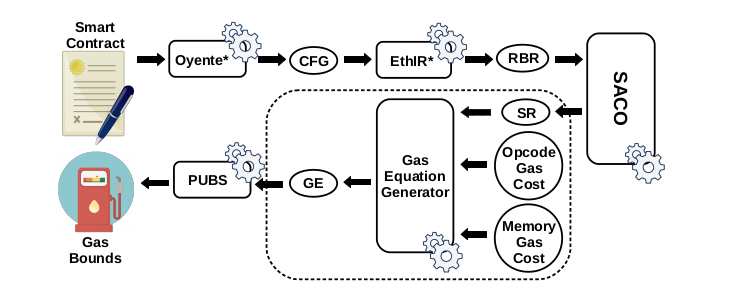
\includegraphics[scale=0.5]{GASTAP-structure.png}
        \caption[Struttura interna di GASTAP]{Architettura di GASTAP}
        \label{fig:gstp-struct}
    \end{figure}
    
    \begin{enumerate}
        \item \textbf{costruzione dei grafi control-flow (CFG)}: tale passaggio è realizzato con \textsc{oyente*}, un'estensione dell'omonimo tool \textsc{oyente} ~\cite{melonproject/oyente}.
        \item \textbf{decompilazione del codice di basso livello}: in questa fase il bytecode viene tradotto in una RBR (\textit{Rule-Based Representation}) grazie ad \textsc{ethir*}, estensione del già citato \textsc{ethir} ~\cite{albert2018ethir}.
        \item \textbf{deduzione delle relazioni di grandezza}: questo passaggio consiste nell'associare a ciascuna delle istruzioni in forma RBR le dimensioni dei dati con i quali interagisce. Quest'operazione è indispensabile per poter costruire le equazioni necessarie a calcolare i bound, e viene realizzata dal tool SACO ~\cite{10.1007/978-3-642-54862-8_46}, che produce le così dette SR (\textit{Size Relations}).
        \item \textbf{generazione delle equazioni di gas}: costituisce il core di GASTAP. Al fine di produrre le equazioni, il tool utilizza le SR insieme alla codifica dei costi delle istruzioni EVM, secondo le specifiche di \cite{wood2014ethereum}. Questi vengono suddivisi tra i costi richiesti dall'esecuzione del bytcode (\textit{Opcode Gas Cost}) e quelli richiesti per l'uso della memoria (\textit{Memory Gas Cost}). 
        \item \textbf{risoluzione delle equazioni fino a formare un bound}: per produrre il risultato finale GASTAP utilizza il solver PUBS ~\cite{albert2008automatic}, che risolve le GE (\textit{Gas Equations}) producendo una formula chiusa dei costi in termini di gas. 
    \end{enumerate}

    \subsection{Interfaccia Web}
    
    GASTAP è utilizzabile tramite un'interfaccia web, disponibile all'indirizzo \\
    https://costa.fdi.ucm.es/gastap.
    
    \begin{figure}[h]
        \centering
        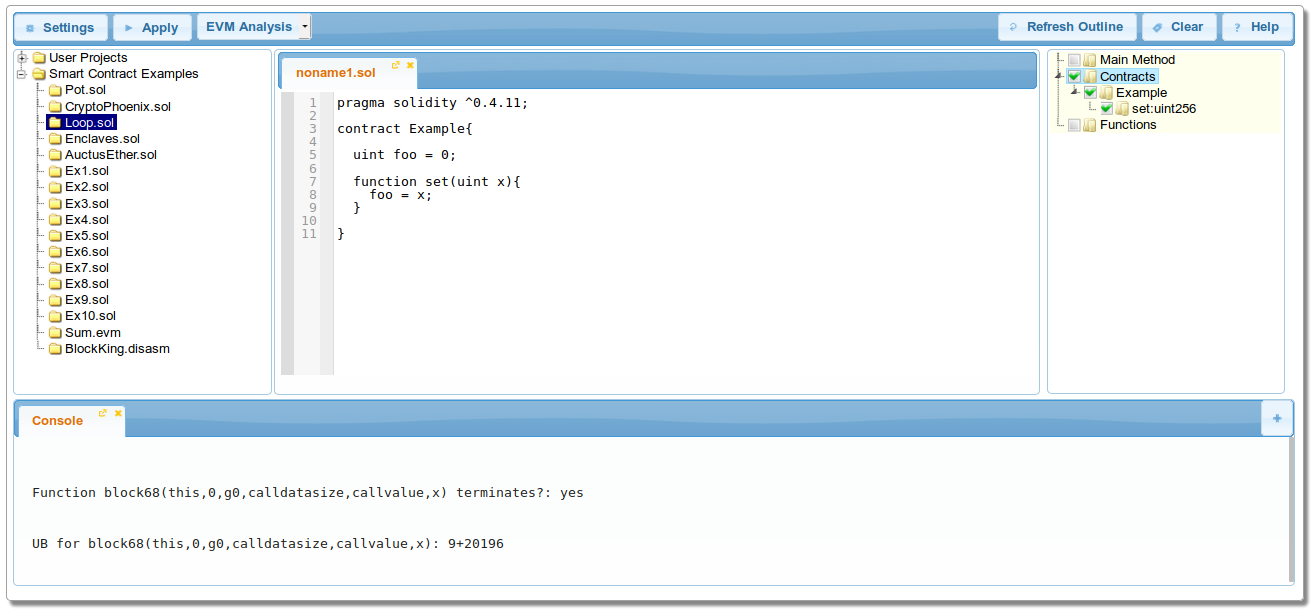
\includegraphics[scale=0.3]{GASTAP-example.png}
        \caption[Interfaccia di GASTAP]{Interfaccia di GASTAP}
        \label{fig:gstp-example}
    \end{figure}
    
    \`E possibile scrivere un proprio programma in Solidity oppure scegliere uno degli esempi proposti dal menù ``Smart Contract Examples''.\newline
    \indent Una volta selezionato il programma di input, cliccando su ``Refresh Outline'' GASTAP mappa le funzioni pubbliche del nostro programma, che vengono mostrate nella sezione di destra. Dopo aver selezionato i metodi che si vogliono analizzare, il pulsante ``Apply'' esegue l'analisi e produce un output nella Console.\newline
    \indent Nell'esempio viene proposto un semplice programma che setta una variabile globale. Stando all'output prodotto, tale programma è garantito teminare, e l'\textit{Upper Bound} (UB) ai consumi di gas è \verb|9+20196|. Si noti che l'upper bound fornito è sempre nella forma \textbf{memory bound} + \textbf{opcode bound}, dove le cifre si riferiscono rispettivamente al bound dei costi di memorizzazione e a quello dei costi delle operazioni che compongono il programma.\newline
